\documentclass{article}

\usepackage{amsmath}
\usepackage{amssymb}
\usepackage{mathtools}
\usepackage{fullpage}
\usepackage[T1]{fontenc}
\usepackage{lmodern}
\usepackage{tikz}
\usetikzlibrary{calc,intersections,through,backgrounds}
\usetikzlibrary{bayesnet}
\usepackage{tikzscale}
\usepackage{tkz-euclide}
\usepackage{tcolorbox}
\tcbuselibrary{skins,breakable}
% pgfplots
\usepackage{pgfplots}
\pgfplotsset{compat=1.8}
% For entities in pgfplots
\newcommand{\entpgf}[1]{\texttt{#1}}

\begin{document}

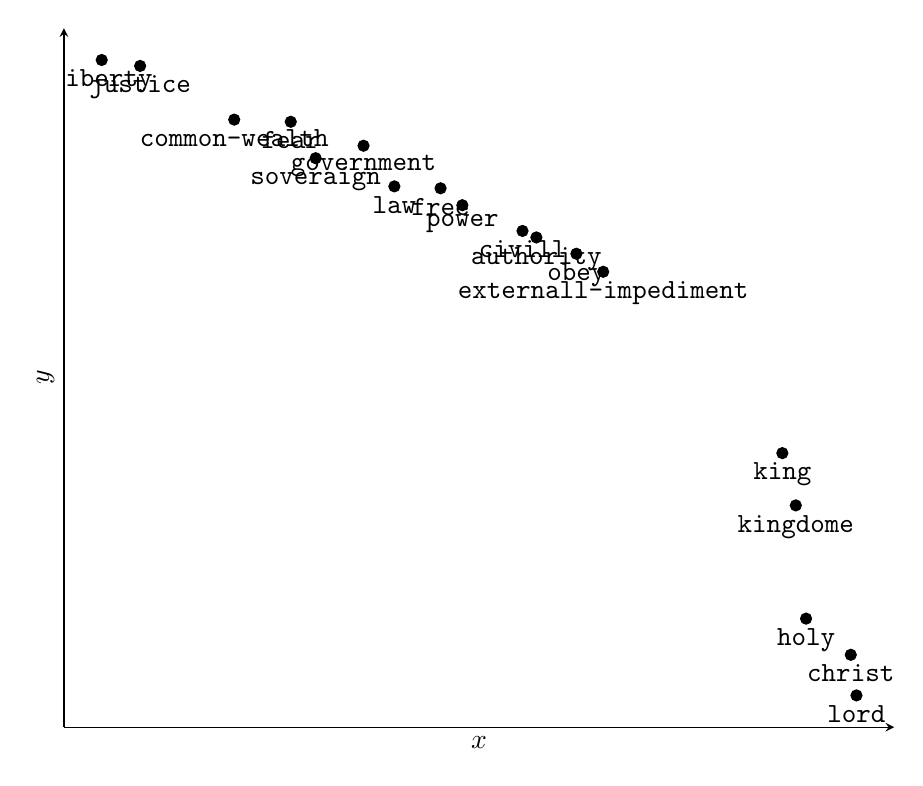
\begin{tikzpicture}
\pgfplotsset{ticks=none}
		\begin{axis}[
		    axis x line=bottom,
			axis y line=left,
			xmin=-6.697371-0.39782998561859134, xmax=1.2592288+0.39782998561859134,
			ymin=-10.214752-0.7001426219940186, ymax=3.7881+0.7001426219940186,
			xtick={-6.697371,1.2592288},ytick={-10.214752,3.7881},
			xlabel=$x$,ylabel=$y$,
			%x label style={anchor=west},
			%y label style={anchor=south},
			width=\textwidth
			]
			\addplot+[mark options={fill=black,color=black},only marks,point meta=explicit symbolic, nodes near coords] coordinates {
(-2.1152288913726807, -0.1221897229552269)[]
(1.1991099119186401, -9.320261001586914)[]
(-2.261406660079956, 0.020989974960684776)[]
(-5.300451755523682, 2.4736626148223877)[]
(-1.4107270240783691, -0.8793035745620728)[]
(-4.704436779022217, 2.4263739585876465)[]
(-3.1251256465911865, 0.9604054689407349)[]
(-3.9373724460601807, 1.898518443107605)[]
(0.728008508682251, -8.522899627685547)[]
(-6.292324542999268, 3.6572659015655518)[]
(0.4779174029827118, -4.875514030456543)[]
(0.6196319460868835, -6.027303218841553)[]
(-3.6122429370880127, 1.0031601190567017)[]
(-6.697371006011963, 3.788100004196167)[]
(1.2592288255691528, -10.214752197265625)[]
(-1.6934442520141602, -0.48169347643852234)[]
(-2.895562171936035, 0.5877139568328857)[]
(-4.442111492156982, 1.623887300491333)[]
};
\node (authority) at (axis cs:-2.115229, -0.12218972){};
\node (christ) at (axis cs:1.1991099, -9.320261){};
\node (civill) at (axis cs:-2.2614067, 0.020989975){};
\node (common-wealth) at (axis cs:-5.3004518, 2.4736626){};
\node (externall-impediment) at (axis cs:-1.410727, -0.8793036){};
\node (fear) at (axis cs:-4.704437, 2.426374){};
\node (free) at (axis cs:-3.1251256, 0.96040547){};
\node (government) at (axis cs:-3.9373724, 1.8985184){};
\node (holy) at (axis cs:0.7280085, -8.5229){};
\node (justice) at (axis cs:-6.2923245, 3.657266){};
\node (king) at (axis cs:0.4779174, -4.875514){};
\node (kingdome) at (axis cs:0.61963195, -6.027303){};
\node (law) at (axis cs:-3.612243, 1.0031601){};
\node (liberty) at (axis cs:-6.697371, 3.7881){};
\node (lord) at (axis cs:1.2592288, -10.214752){};
\node (obey) at (axis cs:-1.6934443, -0.48169348){};
\node (power) at (axis cs:-2.8955622, 0.58771396){};
\node (soveraign) at (axis cs:-4.4421115, 1.6238873){};
\node[anchor = north, xshift=0.0, yshift=0.0] (authorityl) at(axis cs: -2.115229, -0.12218972){$\entpgf{authority}$};
\node[anchor = north, xshift=0.0, yshift=0.0] (christl) at(axis cs: 1.1991099, -9.320261){$\entpgf{christ}$};
\node[anchor = north, xshift=0.0, yshift=0.0] (civilll) at(axis cs: -2.2614067, 0.020989975){$\entpgf{civill}$};
\node[anchor = north, xshift=0.0, yshift=0.0] (common-wealthl) at(axis cs: -5.3004518, 2.4736626){$\entpgf{common-wealth}$};
\node[anchor = north, xshift=0.0, yshift=0.0] (externall-impedimentl) at(axis cs: -1.410727, -0.8793036){$\entpgf{externall-impediment}$};
\node[anchor = north, xshift=0.0, yshift=0.0] (fearl) at(axis cs: -4.704437, 2.426374){$\entpgf{fear}$};
\node[anchor = north, xshift=0.0, yshift=0.0] (freel) at(axis cs: -3.1251256, 0.96040547){$\entpgf{free}$};
\node[anchor = north, xshift=0.0, yshift=0.0] (governmentl) at(axis cs: -3.9373724, 1.8985184){$\entpgf{government}$};
\node[anchor = north, xshift=0.0, yshift=0.0] (holyl) at(axis cs: 0.7280085, -8.5229){$\entpgf{holy}$};
\node[anchor = north, xshift=0.0, yshift=0.0] (justicel) at(axis cs: -6.2923245, 3.657266){$\entpgf{justice}$};
\node[anchor = north, xshift=0.0, yshift=0.0] (kingl) at(axis cs: 0.4779174, -4.875514){$\entpgf{king}$};
\node[anchor = north, xshift=0.0, yshift=0.0] (kingdomel) at(axis cs: 0.61963195, -6.027303){$\entpgf{kingdome}$};
\node[anchor = north, xshift=0.0, yshift=0.0] (lawl) at(axis cs: -3.612243, 1.0031601){$\entpgf{law}$};
\node[anchor = north, xshift=0.0, yshift=0.0] (libertyl) at(axis cs: -6.697371, 3.7881){$\entpgf{liberty}$};
\node[anchor = north, xshift=0.0, yshift=0.0] (lordl) at(axis cs: 1.2592288, -10.214752){$\entpgf{lord}$};
\node[anchor = north, xshift=0.0, yshift=0.0] (obeyl) at(axis cs: -1.6934443, -0.48169348){$\entpgf{obey}$};
\node[anchor = north, xshift=0.0, yshift=0.0] (powerl) at(axis cs: -2.8955622, 0.58771396){$\entpgf{power}$};
\node[anchor = north, xshift=0.0, yshift=0.0] (soveraignl) at(axis cs: -4.4421115, 1.6238873){$\entpgf{soveraign}$};

\end{axis}
\end{tikzpicture}

\end{document}